\documentclass[titlepage,landscape]{seminar}
\usepackage{url}
\usepackage{graphicx}
\usepackage[pdftex]{color}
\usepackage{hyperref}
\usepackage{epstopdf}
\usepackage{slides}
\usepackage{amsmath}

\begin{document}

\myslide{
\begin{eqnarray*}
y_i &=& \mbox{phenotype of inidividual $i$} \\
x_i &=& \mbox{genotypic value of individual $i$} \\
\sigma^2_2 &=& \mbox{environmental variance} \\
\mbox{P}(y_i|x_i) &=& \mbox{N}(x_i, \sigma^2_e)
\end{eqnarray*}
But we don't know $x_i$. We only know the genotype at marker
loci. Suppose we knew that our locus, $Q$ was between $M_1$ and $M_2$
and that the recombination rate between $M_1$ and $Q$ was $r_{1Q}$ and
that the recombination rate between $M_2$ and $Q$ was $r_{Q2}$. Then
\begin{eqnarray*}
\mbox{P}(y_i|M_1,M_2,r_{1Q},r_{Q2},\sigma^2_e) 
&=& \mbox{N}(x_i, \sigma^2_e|M_1,M_2,r_{1Q}r_{Q2})
\end{eqnarray*}
}

\myslide{
\begin{eqnarray*}
P(M_1QM_2/M_1QM_2) &=& \left((1-r_{1Q})(1-r_{Q2})/2\right)^2 \\
P(M_1QM_2/M_1qM_2) &=& 2\left((1-r_{1Q})(1-r_{Q2})/2\right)
                       \left(r_{1Q}r_{Q2}/2\right) \\
P(M_1qM_2/M_1qM_2) &=& \left(r_{1Q}r_{Q2}/2\right)^2
\end{eqnarray*}
\begin{eqnarray*}
P(QQ|M_1M_2/M_1M_2) &= {(1-r_{1Q})^2(1-r_{Q2})^2 \over (1-r_{12})^2} \\
P(Qq|M_1M_2/M_1M_2) &= {2r_{1Q}r_{Q2}(1-r_{1Q})(1-r_{Q2})
                       \over (1-r_{12})^2} \\
P(qq|M_1M_2/M_1M_2) &= {r_{1Q}^2 r_{Q2}^2 \over (1-r_{12})^2} 
\end{eqnarray*}
\[
L(x|M_j) = \sum_{k=1}^N \phi (x|\mu_{Q_k}, \sigma^2) P(Q_k|M_k)
\]
}

\myslide{
\begin{center}
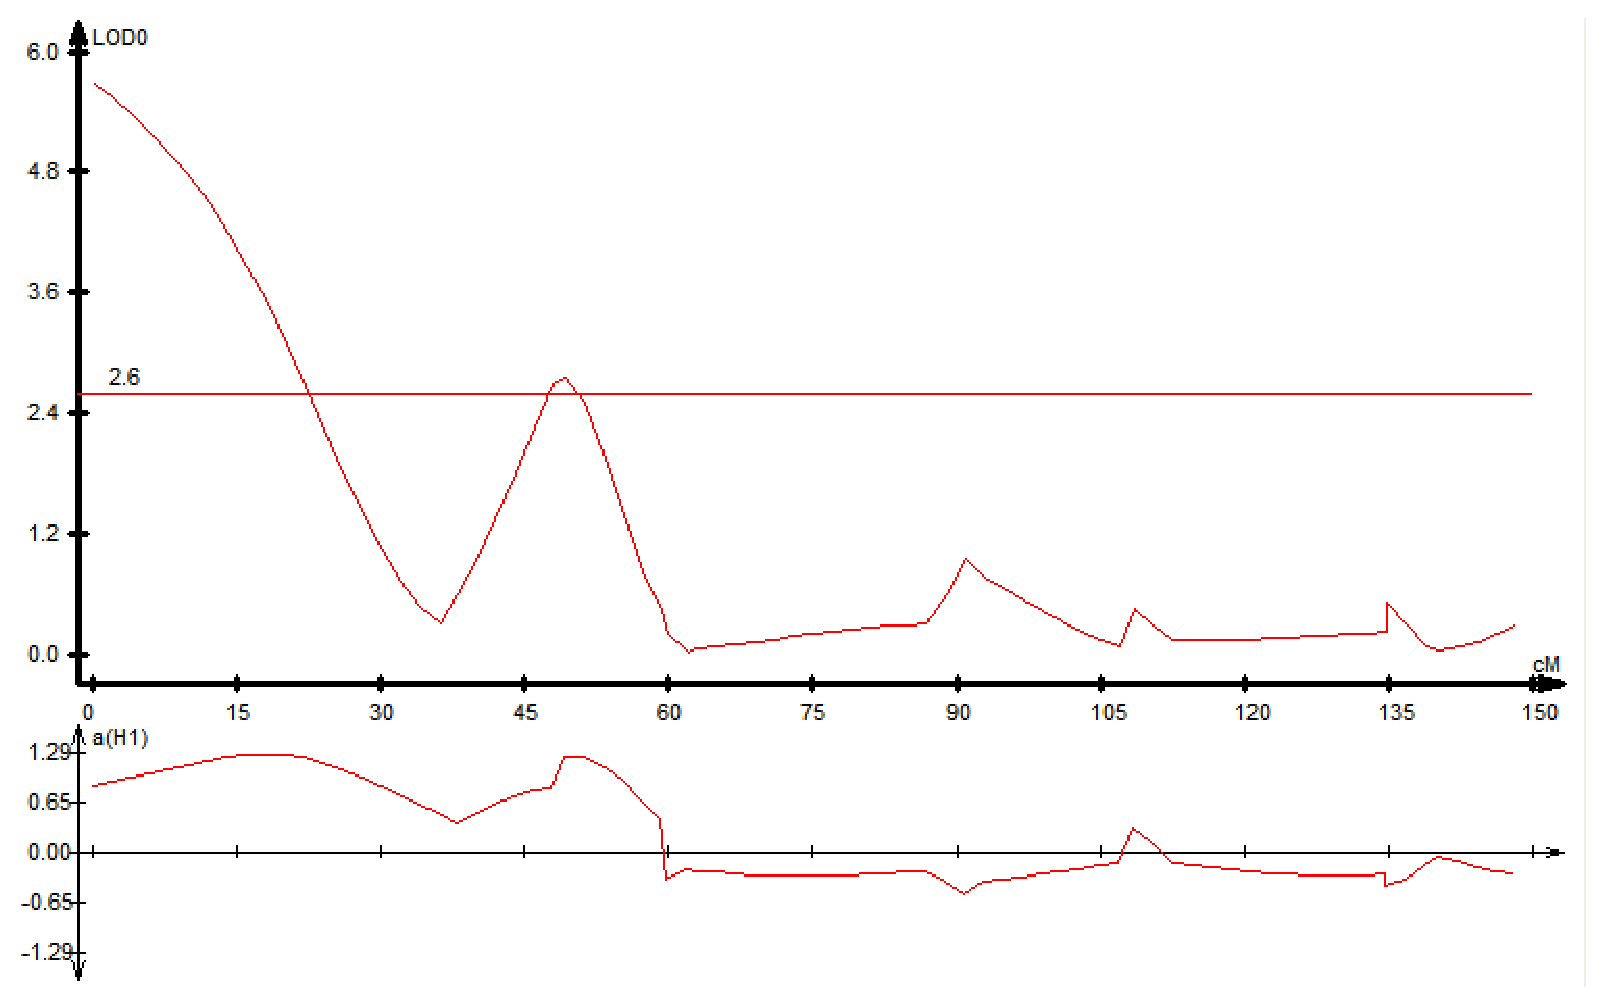
\includegraphics[width=\textwidth]{qtl-composite-results.eps}
\end{center}
}


\myslide{
Alternative approach - a regression:
\[
y_i = \sum_j \beta_jM_j + \epsilon_i \quad ,
\]
where
\[
M_i = \begin{cases}
0 & \mbox{homozygous from ``high'' parent} \\
1 & \mbox{heterozygous} \\
2 & \mbox{homozygous from ``low'' parent}
\end{cases}
\]
\vfil
``Significant'' $\beta_j$ identifies markers associated with
phenotype. 
}

\myslide{
\begin{center}
\begin{tabular}{lcccc}
Gamete    & $A_1B_1$ & $A_1B_2$ & $A_2B_1$ & $A_2B_2$ \\
Frequency & $x_{11}$ & $x_{12}$ & $x_{21}$ & $x_{22}$
\end{tabular}
\end{center}
\vfill
\begin{eqnarray*}
x_{11} &=& p_1p_2 \\
x_{12} &=& p_1q_2 \\
x_{21} &=& q_1p_2 \\
x_{22} &=& q_1q_2
\end{eqnarray*}
\vfill
\begin{eqnarray*}
x_{11} &=& p_1p_2 + D \\
x_{12} &=& p_1q_2 - D \\
x_{21} &=& q_1p_2 - D \\
x_{22} &=& q_1q_2 + D
\end{eqnarray*}
}

\myslide{
\begin{center}
\begin{tabular}{lcccc}
Gamete    & $A_1B_1$ & $A_1B_2$ & $A_2B_1$ & $A_2B_2$ \\
Frequency & $x_{11}$ & $x_{12}$ & $x_{21}$ & $x_{22}$
\end{tabular}
\end{center}
\vfill
\begin{eqnarray*}
x_{11} &=& p_1p_2 + D \\
x_{12} &=& p_1q_2 - D \\
x_{21} &=& q_1p_2 - D \\
x_{22} &=& q_1q_2 + D
\end{eqnarray*}
\vfill
\[D = x_{11}x_{22} - x_{12}x_{21}\]
}

\myslide{
\begin{eqnarray*}
x_{11}' &=& x_{11} - rD \\
x_{12}' &=& x_{12} + rD \\
x_{21}' &=& x_{21} + rD \\
x_{22}' &=& x_{22} - rD
\end{eqnarray*}
\vfill
\[D' = D(1-r)\]
}

\myslide{
\[
\begin{array}{ccccccc}
    &\mu_1            &     &      &     &\mu_2 \\
A_1 &\rightleftharpoons& A_2 &\qquad& B_1 &\rightleftharpoons& B_2 \\
    &\nu_1            &     &      &     &\nu_2 
\end{array}
\]
\vfill
\[
\frac{\mbox{E}(D^2)}{\mbox{E}(p_1(1-p_1)p_2(1-p_2))}
\approx \frac{1}{3 + 4N_er}
\]
}

\myslide{
\begin{center}
\begin{tabular}{c|cccc|cc|c}
\hline\hline
           & \multicolumn{4}{c|}{Gamete frequencies} 
           & \multicolumn{2}{c|}{Allele frequencies} \\
Population & $A_1B_1$ & $A_1B_2$ & $A_2B_1$ & $A_2B_2$ 
           & $p_1$ & $p_2$ & $D$ \\
\hline
1          & 0.24     & 0.36     & 0.16    & 0.24
           & 0.60     & 0.40     & 0.00 \\
2          & 0.14     & 0.56     & 0.06    & 0.24
           & 0.70     & 0.20     & 0.00 \\
Combined   & 0.19     & 0.46     & 0.11    & 0.24
           & 0.65     & 0.30     & -0.005 \\
\hline
\end{tabular}
\end{center}
\vfil
\[
D_t = \mbox{Cov}(p_1,p_2) + \bar D
\]
}

\myslide{
\begin{eqnarray*}
\mbox{\boldmath$y$} &=& \mbox{\boldmath$X$}\beta +
\mbox{\boldmath$Z$}\gamma + \epsilon \\
\mbox{\boldmath$X$} &=& \mbox{how each individual is assigned to a
  genetic grouping} \\
\beta &=& \mbox{mean phenotype of each group} \\
\mbox{\boldmath$Z$} &=& \mbox{genotype of each individual at each
  locus} \\
\gamma &=& \mbox{genotypic effect at each locus} \\
\epsilon &=&  \sim
\mbox{N}(0, \sigma^2\mbox{\boldmath$I$})
\end{eqnarray*}
}

\end{document}



\end{document}

